\documentclass[Journal,letterpaper]{ascelike-new}
%% Please choose the appropriate document class option:
% "Journal" produces double-spaced manuscripts for ASCE journals.
% "NewProceedings" produces single-spaced manuscripts for ASCE conference proceedings.
% "Proceedings" produces older-style single-spaced manuscripts for ASCE conference proceedings. 
%
%% For more details and options, please see the notes in the ascelike-new.cls file.
%
% Some useful packages...
\usepackage[utf8]{inputenc}
\usepackage[T1]{fontenc}
\usepackage{lmodern}
\usepackage{graphicx}
\usepackage[figurename=Fig.,labelfont=bf,labelsep=period]{caption}
\usepackage{subcaption}
\usepackage{amsmath}
%\usepackage{amsfonts}
%\usepackage{amssymb}
%\usepackage{amsbsy}
\usepackage{newtxtext,newtxmath}
\usepackage[colorlinks=true,citecolor=red,linkcolor=black]{hyperref}
%
% Please add the first author's last name here for the footer:
\NameTag{Chen Qi, \today}
% Note that this is not displayed if the NoPageNumbers option is used
% in the documentclass declaration.
%
\begin{document}
% You will need to make the title all-caps
\title{Relationships between individual characteristics and real walking durations from departures to transit stations}
%
\author[1]{Qi Chen}
\author[2]{Shichen Zhao}
%
\affil[1]{Doctor Candidate, Graduate School of Human-Environment Studies, Kyushu University, Japan}
\affil[2]{Professor, Dr. Eng. Faculty of Human-Environment Studies, Kyushu University, Japan}
%
\maketitle

% Please include an abstract:
\begin{abstract}
It is widely accepted that walking durations from departures to transit stations should relate to passengers' individual characteristics. However, since the walking duration is the reflection of the distribution of departure points, maybe it has no simple linear relationship with individual characteristics. Instead of examining the relationship between walking durations and individual characteristics directly, this study examines the feature distribution of individual characteristics over/under several thresholds of walking duration, thus trying to explore this relationship. The rail transit trip survey of Fukuoka, Japan is used as the dataset in this study which includes 4254 records. The features are estimated by using the random forests model. As a result, trip purposes have the most significant effect at any threshold of walking duration; the feature of peak hour also shows importance; the other features have different performance at different thresholds. The result shows a clear relationship between real walking durations and passengers' individual characteristics. Also, this result is expected to provide references for planning the catchment area of transit stations or estimating the catchment area of existing transit stations.
\end{abstract}

%
\section{Introduction}
Mass Rapid Transit (MRT) has been one of the most important parts in public transit system in modern cities. How to shift more people from private car user to public transit passenger is always a key topic for both urban planning and management. There are many factors that can influence the use of public transit, if considering from overall, they can be separated into two parts which are the convenience of public transit (environment factors) and the willingness of traveling by public transit (behavior factors). This study will focus on the behavior factors to examine the relationship between passengers' individual characteristics and walking durations from departures to transit stations.

%
At present, the 800m (half-mile) walking distance has been widely accepted as a principal reference of the catchment area for the planning of Transit-Oriented Development (TOD). Planners and researchers also use transit catchment areas to make prediction of the transit ridership. This 800m walking distance is loosely obtained from the sampling survey that how far people are willing to walk to transit stations, but the same reasoning has been used to justify other transit catchment areas and even in different cities and countries. People with different individual characteristics generally should have different preferences of walking duration, even if they have the same preference of walking duration, their walking distance is not the same because of different walking speeds. It can be assumed that potential public transit users have their own preference and tendency for a given threshold of walking duration. The willingness of using public transit will raise if the expected walking duration is less than the acceptable walking duration, otherwise, the willingness will decrease. Even though the surveyed walking durations should not be viewed as the direct reflection of passengers' willingness for walking durations, they can reflect the differences in the willingness of passengers who have different individual characteristics in an indirect way. On the basis of above-mentioned, this study attempts to give explanations on how individual characteristics influence the walking duration using the study case of Fukuoka subway. The expected result of this study can be viewed as a reflection of willingness for walking durations, and also is expected to provide references for helping determine the catchment area of transit stations.

%
\section{Literature Review}
This section reviews the literature on the issue of walking duration/distance to transit stations, some problems that still not well addressed are collated and summarized. The review is arranged into two parts, how to deal with the variable of walking duration (research object in this study), and how to select the individual characteristics (independent variables in this study).

%
For the walking duration, the research object in this study, there is always a difficult point in obtaining the accuracy walking distance/duration by questionnaire because of the discrepancy between perceived values and objective values \cite{BadlandHannahMandSchofieldGrantMandSchluter2007,McCormack2008}. Also, the observed walking distance/duration is not the reflection of how long people are willing to spend on walking to transit stations, but only the walking distance/duration between the departure and the transit station. For this problem, some studies chose a different perspective trying to explain the walking distance/duration by introducing one threshold of walking duration \cite{Besser2005,McCormack2008}. They examined the differences in the distribution of influencing factors below/above the specific threshold of walking duration. Indeed, using a threshold can decrease the discrepancy between observation and reality in some extent, but this disposal also brought some new problems in. For instance, it may lead to a great loss of information in the raw data, on the other hand, how to decide the threshold is also a key problem. Another problem in this issue is whether to choose walking distance or walking duration as the threshold. To date, there have been a lot of studies working on the relationship between walking distance and passengers' individual characteristics, some of them argued that an individual has a limited amount of time spending on traveling during a day, people tend to accept further walking distance as the speed of travel increases \cite{Marchetti1994,Larsen2010}. That means, passengers with the same individual characteristics may have the similar willingness of walking duration, but they generally have different willingness of walking distance due to different travel speed. This is also the reason why this study chooses the walking duration as the research object.

%
In the influencing factors for walking durations, passengers' individual characteristics are generally thought to be the key that can affect walking distance \cite{Besser2005,WeinsteinAgrawal2008,Krygsman2004,Yang2012,Daniels2013,Guerra2012}, whereas, there are few studies having clearly verified the relationship between individual characteristics and walking distance/duration, even there is a study suggesting the walking distance should not be viewed as a function of socio-demographic characteristics \cite{Krygsman2004}. Several studies have confirmed the role of travel purposes in determining walking distance, the commute trip showed particularity from the other purposes, people with the purpose of commute tend to walk a longer distance to go to transit stations \cite{Larsen2010}. However, the definite relationship between trip purposes and walking distance is still unclear. The same situation is for other categories of factors, such as the factors of transportation environment, land use, and willingness of passengers \cite{Guerra2012,Krygsman2004,WeinsteinAgrawal2008}. The only thing that has been confirmed to date is that the walking distance/duration can be influenced by some specific kinds of factors, such as socio-demographic characteristics, trip purposes, and built-environment, but the problem is how and how much the walking distance/duration can be influenced.

%
In summary, perhaps because of the problems in either the research object or influencing factors, most of the existing studies did not find the significant relevance between the walking distance/duration (research object) and the influencing factors (independent variables). The studies working on the qualitative description for the distribution of walking distance accounted for the majority, although some of the existing studies attempted regression model on this issue, the desired results were not obtained. To avoid such problems mentioned above, this study uses the thresholds of walking duration as the research object. For any given threshold of walking duration, the respondent who gives the answer greater than the given threshold can be viewed as this respondent can accept this threshold of walking duration. The relationship between walking durations and individual characteristics is explained by examining the features of below/above the given thresholds of walking duration. For the analytical method, since various types of regression model has been verified not suitable for this issue, instead of finding the linear relevance between dependent and independent variables, this study introduces the approach of machine learning into this issue, and try to explain the relationship between walking durations and individual characteristics from the view of probability.

%
\section{Data and Methods}

%
\subsection{Introduction for the study case of Fukuoka}
The study case of Fukuoka, is the sixth largest city in Japan which has the largest population in Kyushu Island of Japan (more than 1.5 million). The data source in this study is the Northern Kyushu Area Person Trip, which is conducted about every 12 years, the latest available data is the 4th survey by the year of 2005, and the 5th survey is already in preparation from September 2017. Figure \ref{fig:1} is the research area and the distribution of rail transit stations. By the year of 2005 (the 4th Northern Kyushu Area Person Trip Survey was conducted), there are more than 70 rail transit stations located within the city area of Fukuoka, of which the amount of JR Kyushu stations is 27, Fukuoka Subway is 35, and West Japan Railway is 16. Till now, some new rail transit lines and stations are still under planning and construction. According to the “Survey on the current state of public transportation” published by the Ministry of Land, Infrastructure, Transport and Tourism of Japan, the rail transit system in Fukuoka carries a daily average of more than 0.4 million passengers by 2015 accounting for more than 20\% in total motorized travel. Although the rail transit system of Fukuoka is still not a large-scale one at now, it has been playing a crucial role in people's daily travel.

%
\subsection{Necessary hypothesis}
Based on the ideas outlined above, this study proposes the following three necessary assumption.

\begin{itemize}
\item H1: The distribution of departures and destinations for people with different individual characteristics in Fukuoka, Japan has no significant features in spatial distribution. 

\item H2: The maximum acceptable walking duration of passengers with same individual characteristics should subject to the normal distribution. 

\item H3: The respondents are viewed as they can accept the walking duration that they answered.
\end{itemize}

Based on H1 and H2, if examining the threshold of walking duration $t$, set the proportion of $k$ group in the whole surveyed sample as $r_k$, the proportion of people whose walking durations are less than the given threshold of $t$ minutes is marked as $r_{k}^{<t}$, the proportion of people whose walking durations are more than the given threshold of $t$ minutes is marked as $r_{k}^{>t}$. Now considering if individual characteristics have no significant correlation with maximum acceptable walking durations, there should be no significant differences among $r_k$, $r_{k}^{<t}$, and $r_{k}^{>t}$; otherwise, the three proportion should show significant differences, and the differences will show regular changes at different threshold $t$.

Based on H3, if someone gives the answer $t$ minutes, it means this respondent can accept the walking duration of $t$ minutes and any walking duration that less than $t$ minutes. Indeed, this respondent perhaps can accept the walking duration more than he answered, but in this study, we just concern about if he can accept the given threshold of the walking duration other than how long he can accept.

%
\subsection{Description for the data}
The main purpose of person trip survey is to master the travel trends, thus making a better living environment and providing support for traffic planning. The original data covered the range of all the main cities in Northern Kyushu Area, which has more than 483,000 records of trip chaining behavior. The available data in this study mainly included trip chaining behavior and socio-demographic characteristics, as shown in the table \ref{table:1}.

%
To analyze the walking duration between departure to transit station in Fukuoka, the first step is to extract the valid records of rail transit trip within the city area of Fukuoka from the enormous data of more than 480,000 records. The procedure of extracting the valid data for this study is divided into 3 steps. Firstly, extracting all the person trip data that surveyed within the city area of Fukuoka; secondly, selecting the trip chaining behavior which contains the rail transit mode; thirdly, filtering the invalid data that without null value or abnormal value. The procedure of data cleaning is shown in figure \ref{fig:2}. For analyzing the relationship between walking duration and individual characteristics, only the trip chaining behavior with unique individual identifier can be reserved at last. Finally, the valid dataset is reduced to a size of 4254 trips.

%
Figure \ref{fig:3} shows the age distribution for walking trips to transit stations based on the finally valid dataset. The passengers aged from 25 to 55 account for the major of the whole passengers, while schoolchildren aged under 15 take public transit very little. The distribution graph doesn't show significant peak values at any specific age group. Figure \ref{fig:4} shows the distribution of real walking duration to transit stations, it is generally subject to normal distribution with the mean 8.32, and the standard deviation 2, merely there are several peak values at the time of 5 multiples. It is speculated that the peak values may be caused by deviation occurred in the investigation. Because it seems that people are inclined to reply a looser answer when they are being asked some questions about details. This inclination will count some of the real walking duration that is near to 5 multiples as the 5 multiples and finally expressed in the result of investigation. Despite the existence of differences between survey and reality, as the second assumption proposed above, passengers are viewed that they can accept the walking duration what they answered, therefore, the peak values are thought available in this study.

%
\subsection{Methods}
For the issue of this study, the dependent object is the walking duration to transit stations which is a continuous variable, while the independent objects are multi-categorical variables. An issue like this form is not judged to be suitable for multiple linear regression models. Even the multiple linear regression is the most widely used model for analyzing the relevance of various factors and is also used to estimate the walking duration, the coefficient obtained from the regression model cannot work well on the prediction of walking duration yet \cite{Krygsman2004}. Nevertheless, since what we are concerned with is the threshold of walking duration to transit stations, this issue can be converted into a binary choice problem, which can be also viewed as a classification problem. Giving a specific threshold of walking duration to go to a transit station, people can make the decision of whether choosing the transportation mode of rail transit, and this decision should also be affected by passengers' individual characteristics. That is, if the walking duration of a passenger is longer than a given threshold of walking duration, it can be considered that this given threshold of walking duration is an acceptable one, and he or she may have a relatively high probability of choosing to use rail transit. This willingness or tendency of using rail transit can be reflected by the probabilities of walking longer than the given thresholds. This study will examine the relevance of passengers' individual characteristics and this probability. This probability is used as the dependent variable in this study, given as Equation \ref{eq:1}.

%
\begin{equation}
    D=P^i(t^i>T)
    \label{eq:1}
\end{equation}

%
\begin{description}
    \item[Where:]
    \item[$D$] is the dependent variable,
    \item[$P^i$] is the probability of walking longer than the given threshold for travel individual $i$,
    \item[$t^i$] is the expected walking duration for travel individual $i$.
\end{description}

%
The essence of such kind of binary choice problems is also can be viewed as a classification problem, the models of decision tree, Bayesian, support vector machine (SVM), logistic regression, and neural network are widely adopted for analyzing this kind of problem. In this study, limited by the volume of samples and features, also the unknown for the inner relationship among the features, the decision tree model seems to be a good choice because of the good generalization for different forms of data. Furthermore, to avoid the structure of the tree being too complicated, and to improve the robustness of the model, this study will use an improved model of decision tree, the random forest model, to train and test the samples. Random forests model is an ensemble learning method mainly for classification and prediction. The random forests model is an extension and improvement for the decision tree model, it is operated by constructing a multitude of decision trees and randomly selecting the features at training time \cite{Ho1995,Ho1998}. Another point, for improving the efficiency and accuracy of the model, also reducing the number of invalid branches in the model, it is necessary to filter the invalid features before estimating the model.

%
Briefly, the general process of this study can be summarized as follows. Data is extracted on the Fukuoka city-wide, including 4254 samples, and 6 main categories of features. The features with importance in explaining the willingness of walking duration are selected by using analysis of variance (ANOVA). Then random forest model for each threshold of walking duration is estimated. Finally, the result obtained from the random forest model can be used for predicting the probability of people walking to transit station within a specific threshold of walking duration.

%
\section{Feature selection}
The procedure of feature selection includes two parts, the first is the disposal of features with low variance, and the second is the univariate feature selection. The first one is used for filtering the features accounting for very little in the total samples, because a too small quantity cannot present significant influence on the result. In this study, the multi-categorical features in the original dataset are reclassified into some larger groups, thus dealing with the features with low variance. The second step is to select the valid features that indeed have relevance with the independent variable, this step is processed based on statistical tests. In this study, the Analysis of Variance (ANOVA) is used for estimating the importance of each feature.

%
\subsection{Reclassifying features}
The feature of trip purpose has 15 subcategories in the original dataset, this study reclassifies it into commuting to work, commuting to school, official business, private purpose (such as shopping, entertainment), and going home, 5 categories. The feature of occupation is reclassified from 14 subcategories into 5 categories as well, they are service, technology, administration, student, and the other. Table \ref{table:2} reports some of the statistical description for each feature. Overall, the average walking duration to transit stations is 8.32 minutes, more than 75\% are less than 10 minutes, most people walk to transit stations costing 5-10 minutes. In detail, there are some significant differences in the statistical description for each feature, the differences are summarized as follows.

%
\begin{enumerate}
    \item The walking duration in peak hour is longer than off peak hour.
    \item Young and old people are inclined to spend less time on walking to transit stations.
    \item Trips with purposes of official business and going home tend to take shorter time in walking to transit stations.
    \item Walking trips for commuting to work are significantly longer than walking trips for other purposes.
\end{enumerate}

%
\subsection{Univariate feature selection}
According to the achievements from previous studies, the walking distance to transit stations ranged generally from 400 meters to 1000 meters in terms of different city types, travel habits, and even the needs of research purpose \cite{Guerra2012,Murray1998,OSullivan1996,Keijer2000,Zhao2003,Alshalalfah2007}. If converting this walking distance into walking duration by calculating the walking speed of 4.8 km/h, which has been argued in the existing study \cite{Bohannon1997}, the walking duration would range from 5 minutes to 13 minutes. Back to this study, more than 40\% of the walking duration are less than 5 minutes, and the walking duration within 13 minutes covers about 85\% of the total. The 5 minutes’ range can be viewed as the acceptable walking duration of the main users of transit stations, while a walking duration longer than 13 minutes cannot be accepted by most of the rail transit users. In addition, the mean walking duration in this study is about 8 minutes, therefore, the three more representative thresholds of 5, 8, 13 minutes are picked as the typical threshold for estimating the relationship between individual characteristics and walking durations. The features with significance in explaining the walking duration (the p-value in ANOVA less than 0.05, which means this feature relevant with the dependent variable at the confidence level of 95\%) are picked out and listed in Table \ref{table:3}.

%
For the threshold of 5 minutes, the features of trip purposes and peak hour play the most important role in determining the willingness of walking duration. Situations are changed a little in the case of 8 minutes, the importance of age and sex raised in some extent, while the features of trip purposes change little from that of 5 minutes. For the threshold of 13 minutes, the feature importance shows a big difference from 5 and 8 minutes. This result of feature selection is also consistent with known characteristic of rail transit use. Most of the walking duration is distributed around the average walking duration 8 minutes, it can be considered that walking duration between 5 and 13 minutes is sensitive to individual characteristics. The walking duration more than 13 minutes is not accepted by most people even if they have different individual characteristics, and the threshold less than 5 minutes is also not sensitive to individual characteristics since the 5 minutes threshold is a generally acceptable one for most passengers.

%
\section{Estimation of features}
The valid features (Table \ref{table:3}) are used in the random forest model to estimate the probability of walking longer than the given threshold of walking duration in terms of people with different characteristics. For estimating the model, the dataset is divided into two parts, 50\% of the samples are used for fitting the model and obtaining the coefficients, the rest 50\% are used for testing the ability of prediction. The probabilities of walking less than the given threshold of walking duration can be estimated by the decision tree obtained by the random forest model, the prediction process based on the decision tree from the random forest model is presented in Figure \ref{fig:5}. The prediction in random forest model is not obtained from the only one decision tree but the multitude of decision trees constructed by random selection of features and samples. Finally, the dependent variable at the given threshold of walking duration to transit stations is calculated by equation \ref{eq:1} based on the mean prediction.

%
The accuracy of results are evaluated by using the method of simple moving average. Figure \ref{fig:6} is the trend line of probabilities of walking less than the given threshold. 
The trend line of the surveyed values based on the test set is calculated by the mean probability of a group people who have close predicted values. The trend line is drawn by a descending order of predicted values. From the comparison of predicted values and surveyed values, it can be known that the prediction at the threshold of 5 minutes has the best fitness, and the prediction for the threshold of 13 minutes is also slightly good, while it’s not so good in the case of 8 minutes. In fact, if checking the prediction for individuals, the accuracy of this model is still not enough to explain the individual behavior. But trend line shown in Figure \ref{fig:6} partly proved that this result can be used for reflecting the behavior of a group of people at a given threshold of walking duration. Here the discrepancy occured between the surveyed data and realities, but in this study

%
\section{Discussion and Conclusion}
This study described and analyzed more than 4200 samples for the trips of rail transit. Three thresholds of walking duration are examined. From the result of Table \ref{table:3}, trip purpose is the most important factor in determining the walking durations at all the 3 thresholds. The feature of peak hour is also significant in explaining the walking duration. People can accept a longer time to go to stations at peak hours, while people with private purpose or on the way going home are not willing to choose the stations far away. For the details of each threshold, the unemployed people and the elderly people tend to walk less than 5 minutes for accessing transit stations; it is a little difficult for females and the people whose age is between 25 and 44 to accept a walking duration more than 8 minutes; the people whose age is between 45 to 64 can accept the walking duration of more than 13 minutes more easily than the others.

%
But what summarized above is only the description for the distribution of walking duration in terms of each feature. Even knowing these, it is difficult to make use of them, just as the achievement obtained by previous studies. In fact, the data in this study is obtained from a factual investigation but not a willingness survey. Once people have made a decision of walking to transit stations, the real explanation of walking duration is the location of departure and the walking speed. It is hard to say whether the individual characteristics affected the walking durations. Therefore, for this kind of study, the two assumptions proposed above are necessary. If a passenger chose to walk to a transit station, it means this passenger can accept the walking duration from his/her departure to that transit station. The distribution of walking durations for each group of people with a specific feature can be considered as the reflection of the acceptable walking duration for that group of people. Perhaps due to the reasons of discrepancy in investigation and the basic assumption, few existing studies can explain the relevant between walking duration and individual characteristics quantitatively correctly.

%
According to the achievement of previous studies, if examining the walking duration as a continuous variable, there is no linear relation between walking duration and individual characteristics. For this reason, this study tried to explain the walking duration by examining some specific threshold. As the results, the model of 5 minutes’ threshold has a better explanatory power, the model of 13 minutes' threshold is a little weak, and the model of 8 minutes' threshold is not good. Here are some possible reasons for explaining the results. The selected thresholds of walking duration 5, 8, 13 minutes represent the lower boundary, mean value, and upper boundary of the major distribution of walking durations respectively. The acceptable walking durations range from 5 to 13 minutes, therefore, it can be inferred that people who prefer walking less than 5 minutes and who can accept walking longer than 13 minutes may have significant features. However, as the mean value of walking duration, it can be thought that most of the walking durations are distributed around 8 minutes, for passengers there may be some randomness in making the decision of whether walking to transit stations. For the other threshold values near the mean value of 8 minutes, it also can be inferred that people may have some ambiguity in choosing whether to walk to transit stations or not. This explanation can also be partly confirmed by the result of valid features selection. There are 5 identical features in both thresholds of 5 and 8 minutes, which means people with those features are not sensitive to the threshold from 5 to 8 minutes.

%
Overall, the results of the random forest model perform not well on individual predictions. But for the average probability of a group of people, it shows a good predictive ability at the threshold of 5 minutes. In the next stage of this research, we plan to apply the results on predicting the willingness at a specific threshold of walking duration for a group of people. Also, the results can be used in planning the catchment area of transit stations or estimating the catchment area of existing transit stations.


% Appendix for all the tables and figures

% Here are the tables
%
\begin{table}[htbp]
    \centering
    \caption{Available Data Contents}
    \label{table:1}
    \begin{tabular}{cl}
    \hline\hline
      Category                      & Feature\\
    \hline
      Trip chaining behavior        & Departure location \\
                                    & Departure time \\
                                    & Destination location \\
                                    & Arrival time \\
                                    & Transport modes \\
                                    & Time spent for each mode \\
                                    & Location of bus stop or rail transit station \\
      Socio-demographic attributes  & Age \\
                                    & Sex \\
                                    & Occupation \\
                                    & Trip purpose \\
                                    & Vehicle/License holding \\
                                    & Address \\
    \hline\hline
    \end{tabular}
    \normalsize
\end{table}
%

\begin{table}[htbp]
    \caption{Statistical Description of Walking Duration for Each Feature}
    \label{table:2}
    \centering
    \small
    \renewcommand{\arraystretch}{1.25}
    \begin{tabular}{llrrccccccc}
        \hline\hline
 Features & Categories & Count & Percentage & Mean & Std & 10th & 25th & 50th & 75th & 90th\\
        \hline
 & Total    & 4254  & -         & 8.32  & 4.63  & 3     & 5     & 8     & 10    & 15 \\
 &          &       &           &       &       &       &       &       &       & \\
%
        \multicolumn{1}{l}{Sex}
 & male     & 2257  & 53.1\%    & 8.41  & 4.63  & 3     & 5     & 8     & 10    & 15 \\
 & female   & 1996  & 46.90\%   & 8.22  & 4.63  & 3     & 5     & 7     & 10    & 15 \\
%
        \multicolumn{1}{l}{Peak hour}
 & peak     & 2976  & 70.00\%   & 8.51  & 4.66  & 3     & 5     & 8     & 10    & 15 \\
 & Off peak & 1277  & 30.00\%   & 7.88  & 4.52  & 3     & 5     & 7     & 10    & 15 \\
%
        \multicolumn{1}{l}{Age}
 & 5-24     & 543   & 12.80\%   & 8.18  & 4.7   & 3     & 5     & 7     & 10    & 15 \\
 & 25-44    & 1992  & 46.80\%   & 8.36  & 4.42  & 3     & 5     & 8     & 10    & 15 \\
 & 45-64    & 1407  & 33.10\%   & 8.43  & 4.83  & 3     & 5     & 8     & 10    & 15 \\
 & 65-      & 311   &  7.30\%   & 7.78  & 4.81  & 3     & 5     & 7     & 10    & 15 \\
%
        \multicolumn{1}{l}{Occupation}
 & service  & 1256  & 29.50\%   & 8.32  & 4.57  & 3     & 5     & 8     & 10    & 15 \\
 & tech     & 721   & 17.00\%   & 8.58  & 4.89  & 3     & 5     & 8     & 10    & 15 \\
 & office   & 1076  & 25.30\%   & 8.44  & 4.48  & 4     & 5     & 8     & 10    & 15 \\
 & student  & 325   &  7.60\%   & 8.12  & 4.73  & 3     & 5     & 7     & 10    & 15 \\
 & null     & 875   & 20.60\%   & 8.03  & 4.62  & 3     & 5     & 7     & 10    & 15 \\
%
        \multicolumn{1}{l}{Purpose}
 & commuting to work   & 2697  & 63.40\% & 8.69  & 4.51  & 4     & 5     & 9     & 10    & 15 \\
 & commuting to school & 287   &  6.70\% & 8.19  & 4.6   & 3     & 5     & 8     & 10    & 15 \\
 & official business   & 153   &  3.60\% & 7.1   & 5.05  & 2     & 3     & 5     & 10    & 15 \\
 & private purpose     & 789   & 18.60\% & 7.82  & 4.78  & 3     & 5     & 7     & 10    & 15 \\
 & going home          & 327   &  7.70\% & 7.17  & 4.67  & 2     & 5     & 5     & 10    & 15 \\
%
        \hline\hline
    \end{tabular}
    \normalsize
\end{table}

%
\begin{table}[htbp]
    \caption{Valid Features and the Effect at Each Threshold}
    \label{table:3}
    \centering
    \begin{tabular}{lrlrlr}
    \hline\hline
    \multicolumn{2}{c}{5 min threshold} & \multicolumn{2}{c}{8 min threshold} & \multicolumn{2}{c}{13 min threshold} \\
    \hline
Features 	& Effect* 	& Features 	& Effect*		& Features 	& Effect* \\
Age over 65 			& L	& Female				& M	& Age 45-64				& M	\\
Peak hour				& M	& Age 25-44 			& M	& Peak hour 			& M	\\
O\_Null					& L	& Peak hour				& M	& P\_commuting to work 	& M \\
P\_commuting to work	& M	& P\_commuting to work  & M	& P\_ private purpose 	& L \\
P\_official business	& L & P\_official business	& L	&       				&  	\\
P\_private purpose		& L & P\_ private purpose	& L &       				&  	\\
P\_going home 			& L & P\_ going home 		& L &       				&   \\
    \hline\hline
    \end{tabular}
    \normalsize
%
    \begin{description}
        \label{note:1}
        \item[*Note:]
L means the individual with this feature tend to spend less time than the given threshold of walking duration on accessing transit stations, while M is the opposite meaning.
        \end{description}
\end{table}

%
% Here are the figures
\begin{figure}[htp]
    \caption{Distribution of Transit Stations}
    \label{fig:1}
    \centering
    \fbox{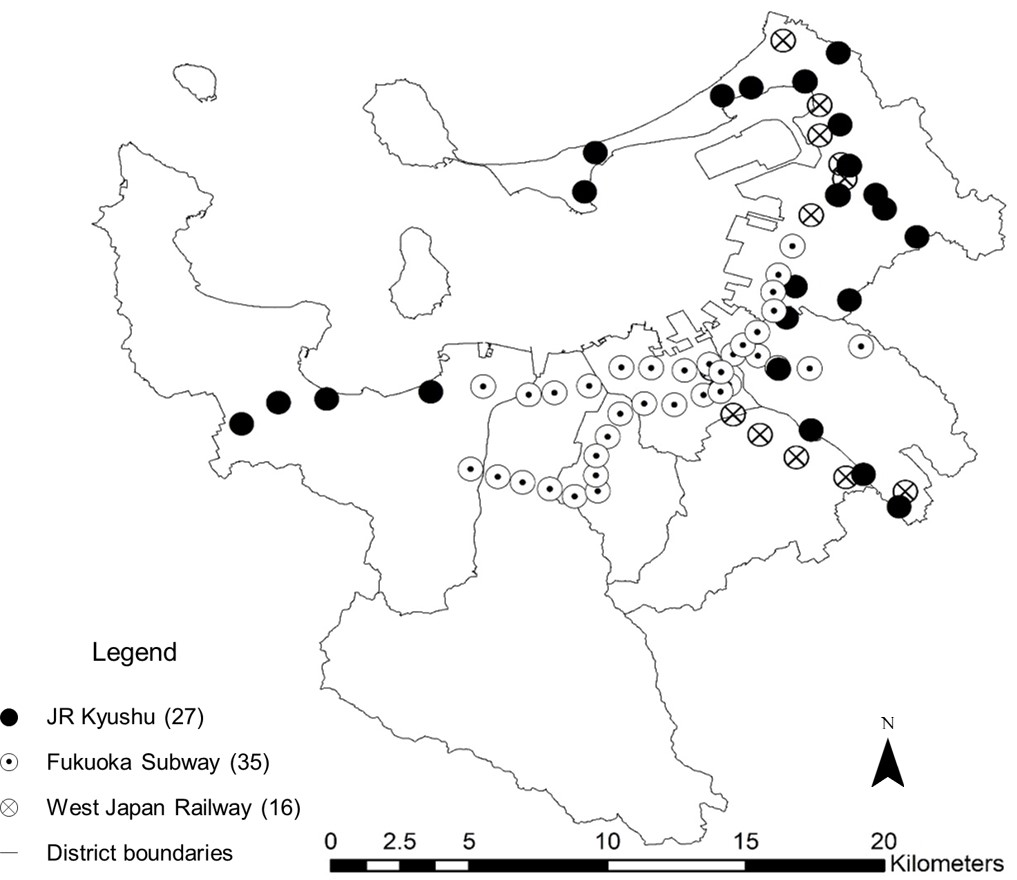
\includegraphics[width=1\linewidth]{fig1}}
\end{figure}

%
\begin{figure}[htp]
    \caption{Process of Data Cleaning}
    \label{fig:2}
    \centering
    \fbox{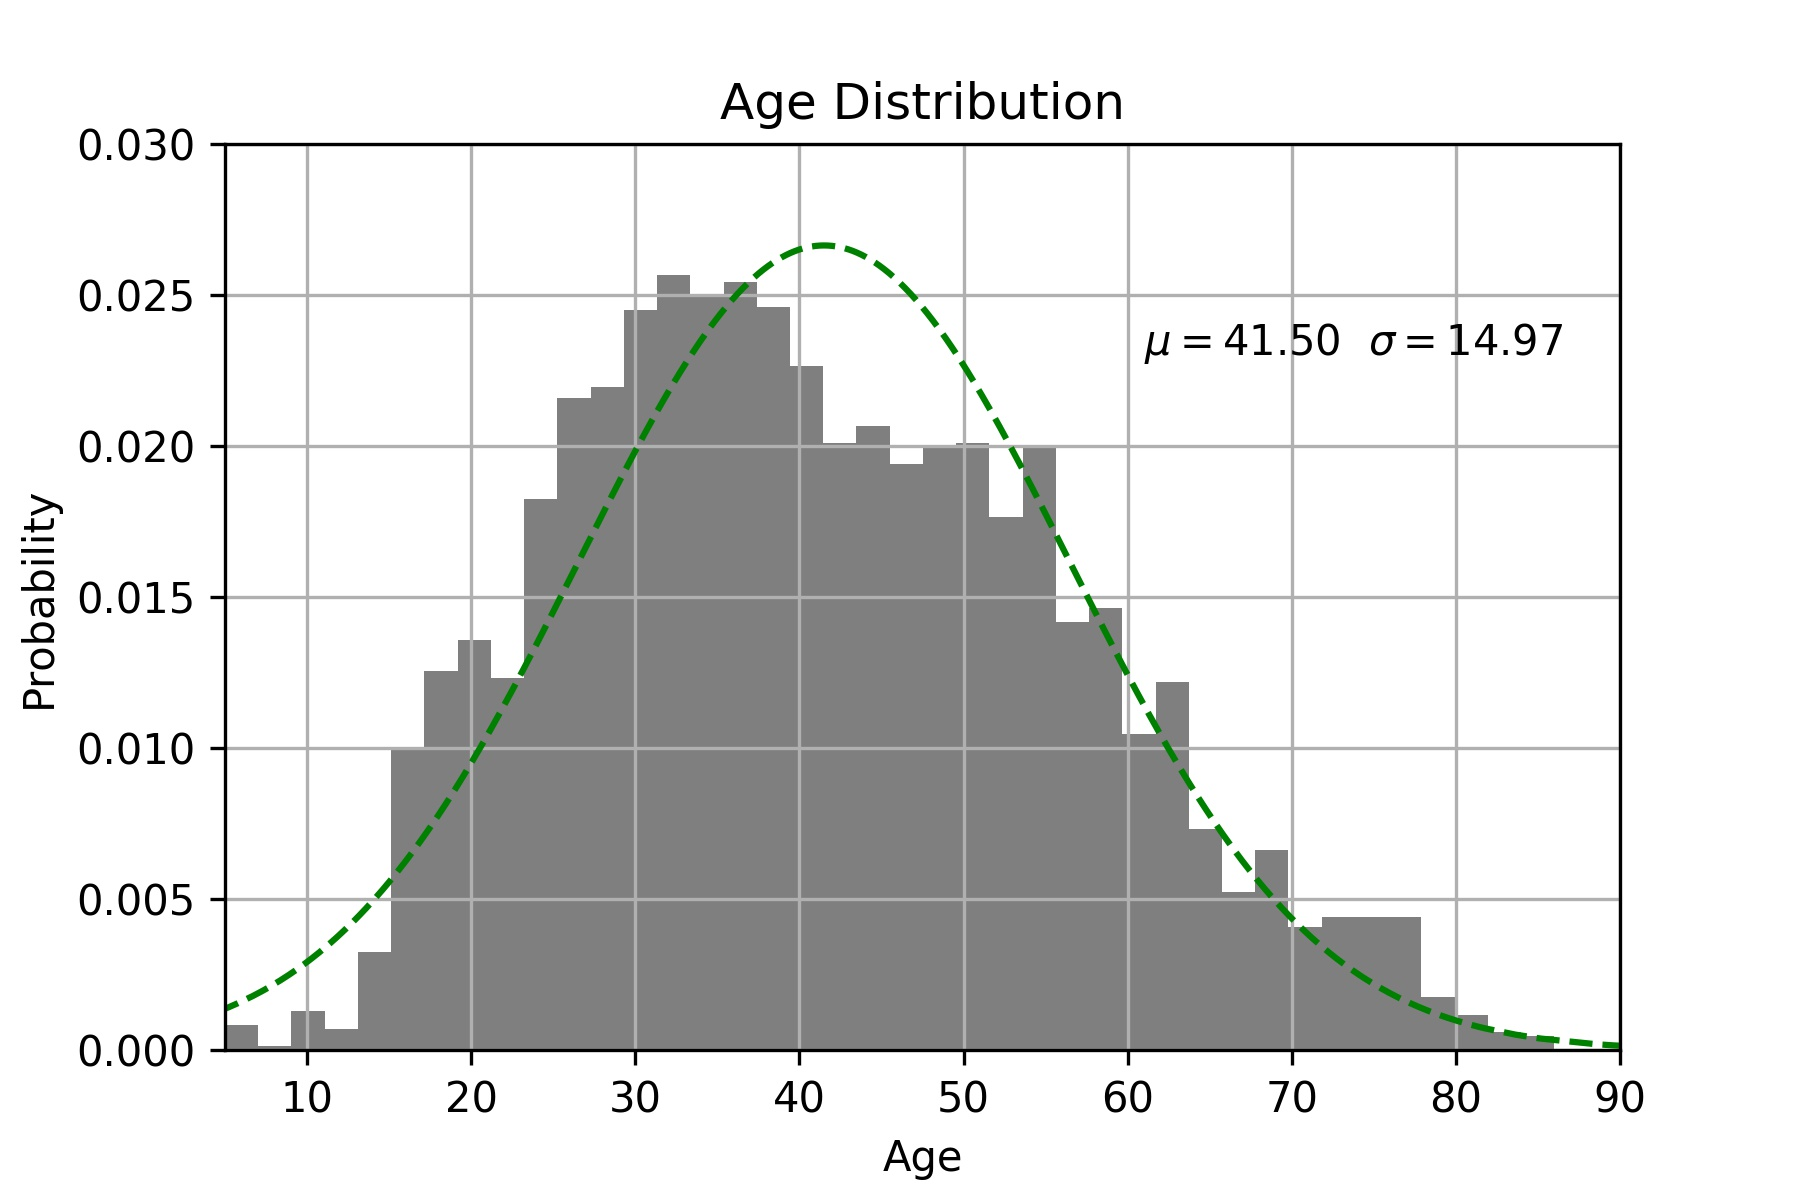
\includegraphics[width=1\linewidth]{fig2}}
\end{figure}

%
\begin{figure}[htp]
    \caption{The Age Distribution of Passengers}
    \label{fig:3}
    \centering
    \fbox{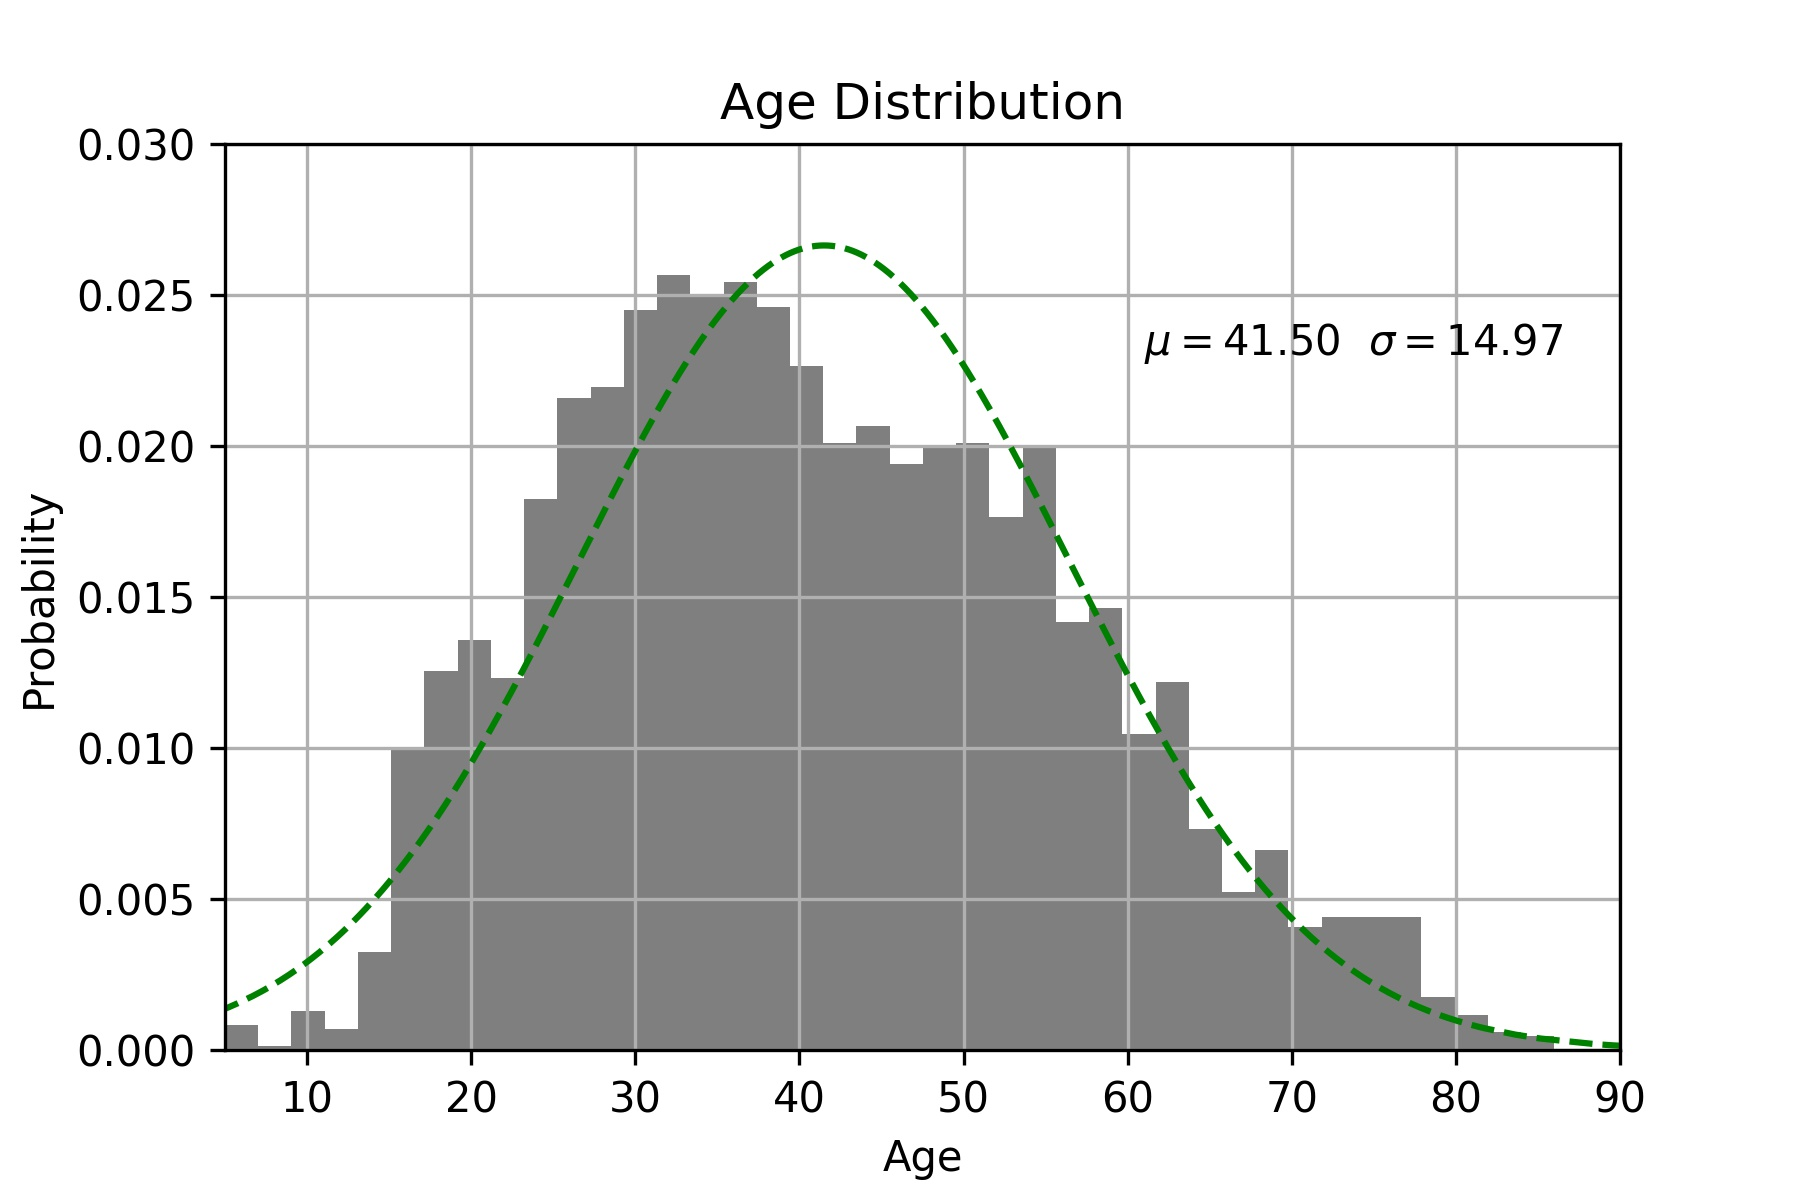
\includegraphics[width=1\linewidth]{fig3}}
\end{figure}

%
\begin{figure}[htp]
    \caption{Distribution of Walking Duration}
    \label{fig:4}
    \centering
    \fbox{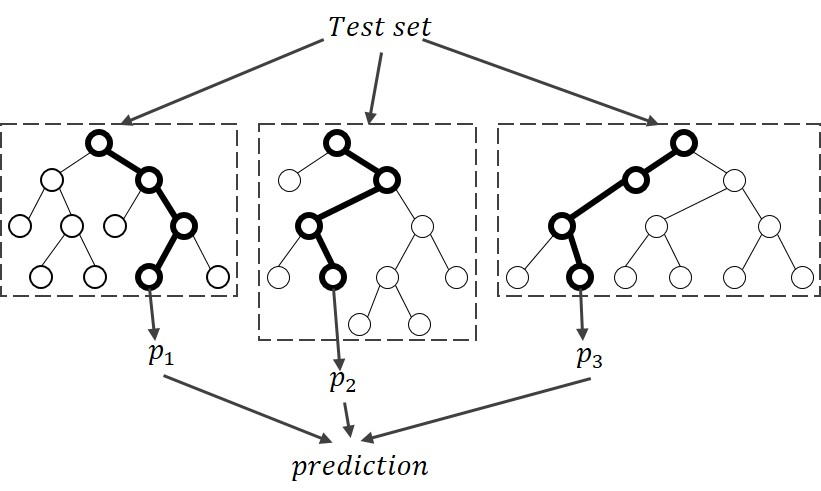
\includegraphics[width=1\linewidth]{fig4}}
\end{figure}

%
\begin{figure}[htp]
    \caption{Prediction Process in Random Forests Model}
    \label{fig:5}
    \centering
    \fbox{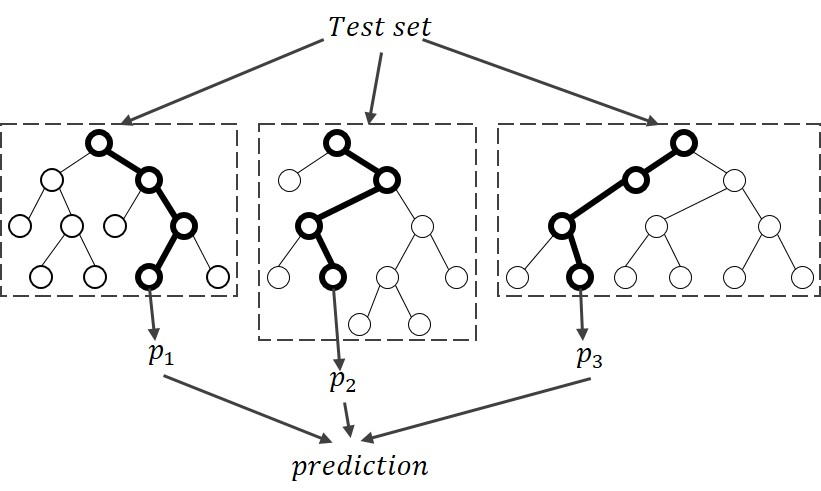
\includegraphics[width=1\linewidth]{fig5}}
\end{figure}

%
\begin{figure}[htp]
    \caption{Trend Line of Prediction and Test Set}
    \label{fig:6}
    \centering
    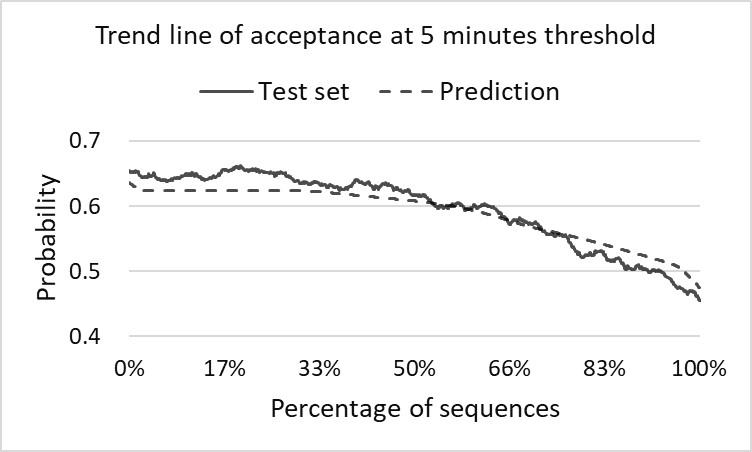
\includegraphics[width=0.7\linewidth]{fig6-1}\\
    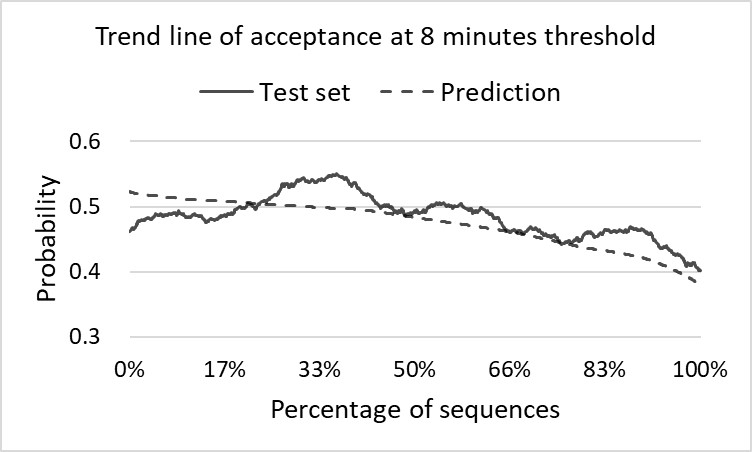
\includegraphics[width=0.7\linewidth]{fig6-2}\\
    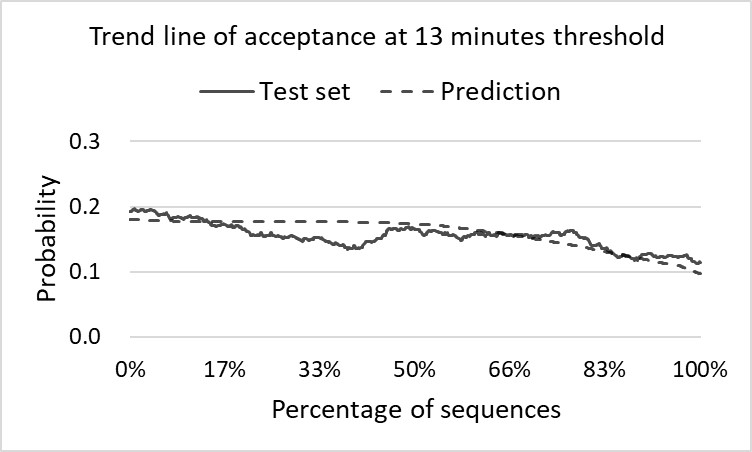
\includegraphics[width=0.7\linewidth]{fig6-3}\\
\end{figure}

% Format setting
\pagebreak

%
\bibliography{ascexmpl-new}

%
\end{document}
